\documentclass[11pt, oneside,a4paper]{article}
%\usepackage[margin=1.75in]{geometry}

\usepackage{hyperref}
\usepackage{graphicx}
\usepackage{array}

\renewcommand{\thesubsection}{\thesection.\alph{subsection}}
\newcommand{\artichoke}[1]{
\includegraphics[width=#1]{images/artichoke-clr.png}}
\newcommand{\artichokeBW}[1]{
\includegraphics[width=#1]{images/artichoke-bw.png}}
\newcommand{\thumbs}[1]{
\includegraphics[width=#1]{images/thumbs.png}}
\newcommand{\bowl}[1]{
\includegraphics[width=#1]{images/bowl.png}}
\newcommand{\pizza}[1]{
\includegraphics[width=#1]{images/pizza.png}}

\title{Proposal for Emoji: Artichoke }

\author{Ethan Mahintorabi \\ emahintorabi@gmail.com 
\and Anna Starr \\ annacstarr@gmail.com}

\begin{document} 
\maketitle 

\newcolumntype{P}[1]{>{\centering\arraybackslash}p{#1}}
  \begin{table}[h]
    \centering
    \begin{tabular}{P{1cm}P{3cm}P{3cm}}
    \hline
      Size & Black \& White & Color \\ \hline
      72px & \artichokeBW{72px} & \artichoke{72px} \\ \hline
      18px & 
\includegraphics[width=18px]{images/artichoke-bw.png} & \artichoke{18px} \\ \hline
    \end{tabular}
    \caption{All images are offered under CC0 by the author Ethan Mahintorabi.}
    \label{my-label}
  \end{table}

  \section{Identification}
    \textbf{CLDR} short name \textbf{--} \texttt{artichoke} \\
    \textbf{CLDR} keywords \textbf{--} \texttt{artichoke | vegetable | thisle}
   
  
  \section{Images}
  Images are provided in Table \ref{my-label}. With all variants offered under CC0.

  \section{Sort Location}
    \textbf{Category} \textbf{--} \texttt{food-vegetable} \\
    \textbf{Order} \textbf{--} After BROCCOLI
  
  \section{Reference Emoji}
    The reference emoji chosen for comparison is MELON FOOD. 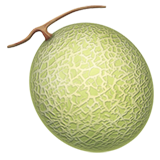
\includegraphics[width=18px]{images/melon.png}

  \newpage


  \section{Selection Factors -- Inclusion}
    \subsection{Compatability}
    \textbf{n/a}

    \subsection{Expected Usage Level}
      \subsubsection{Frequency}
        \paragraph{}
        Google Search (English) \\
        
\includegraphics[width=350px]{google_english/artichoke.png}\\
        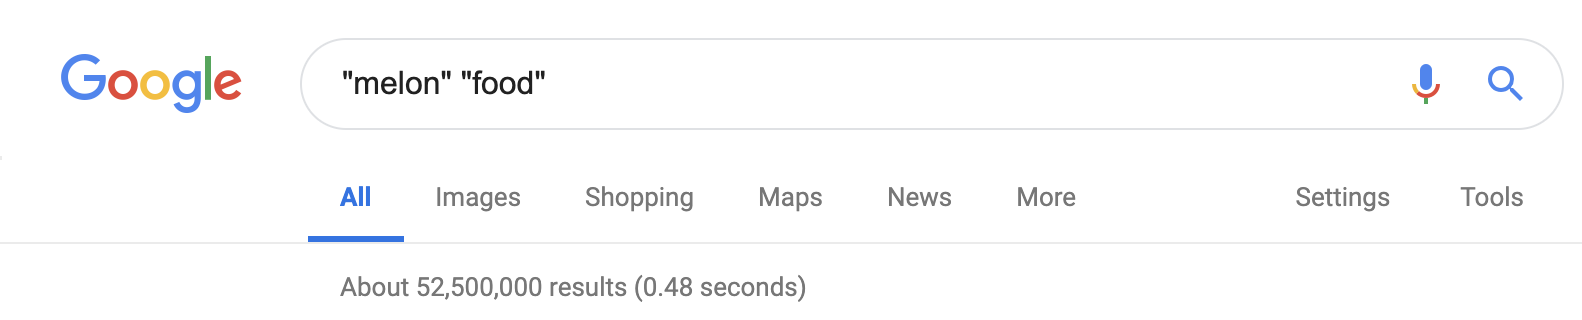
\includegraphics[width=350px]{google_english/melon.png}

        \vspace{1.5 cm}

        \paragraph{}
        \noindent Bing Search (English) \\
        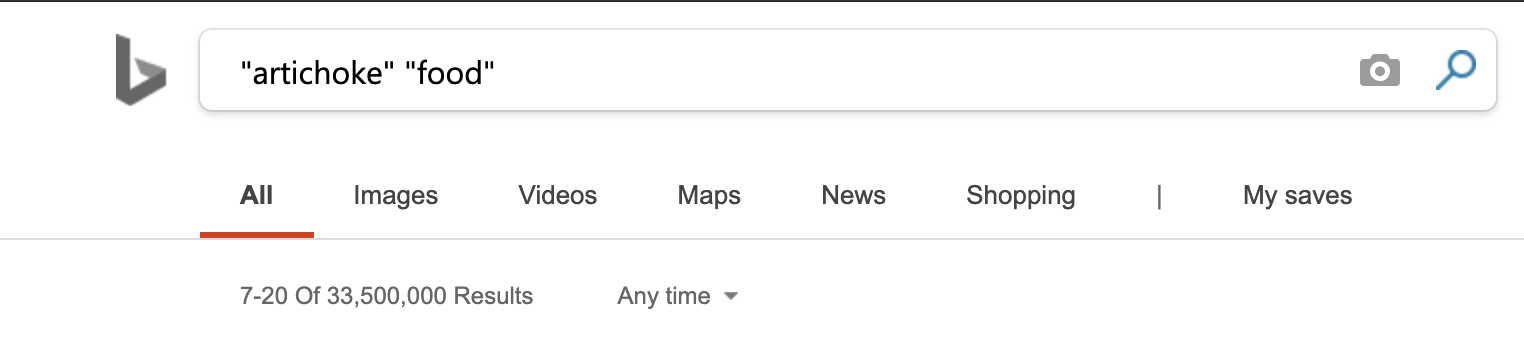
\includegraphics[width=350px]{bing_english/artichoke.png}\\
        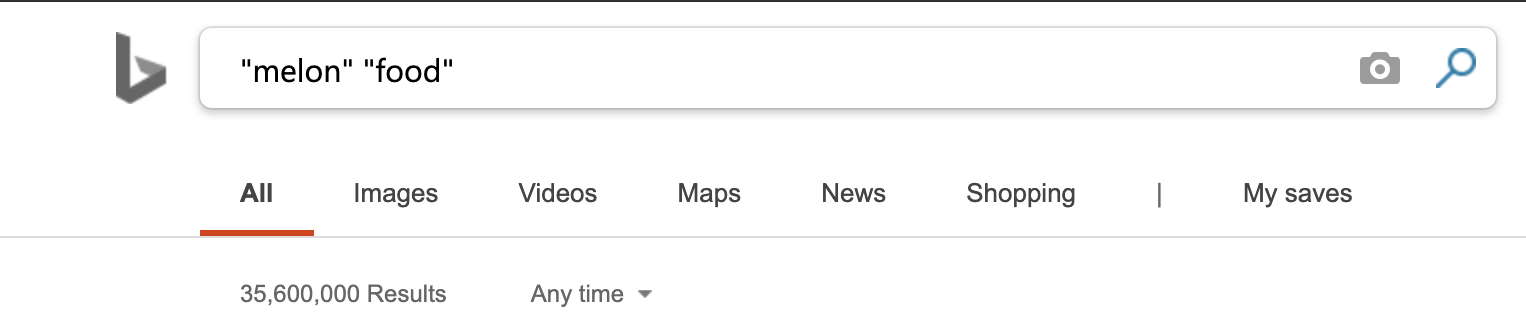
\includegraphics[width=350px]{bing_english/melon.png}

        \vspace{1.5 cm}
        
        \paragraph{}
        \noindent YouTube Search (English) \\
        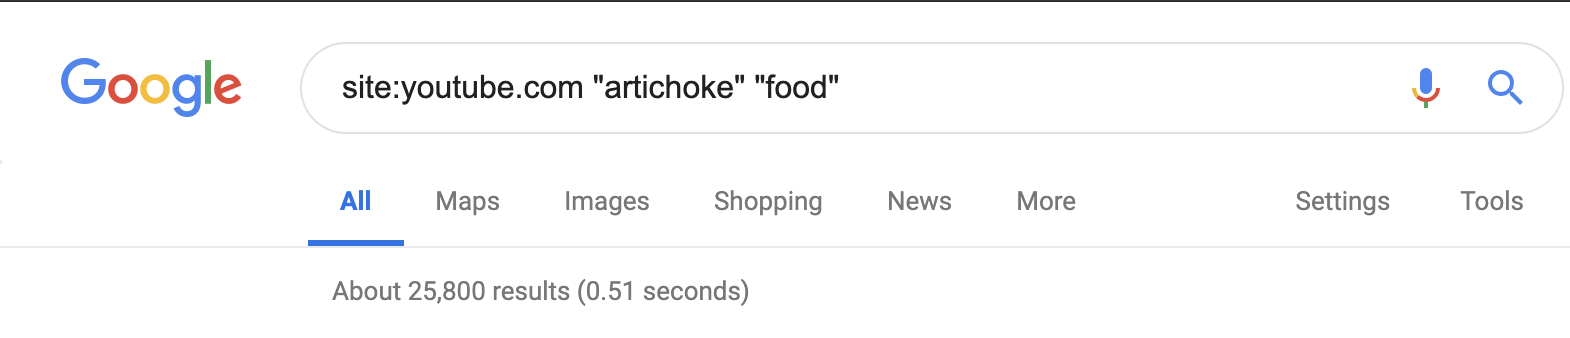
\includegraphics[width=350px]{youtube/artichoke.png}\\
        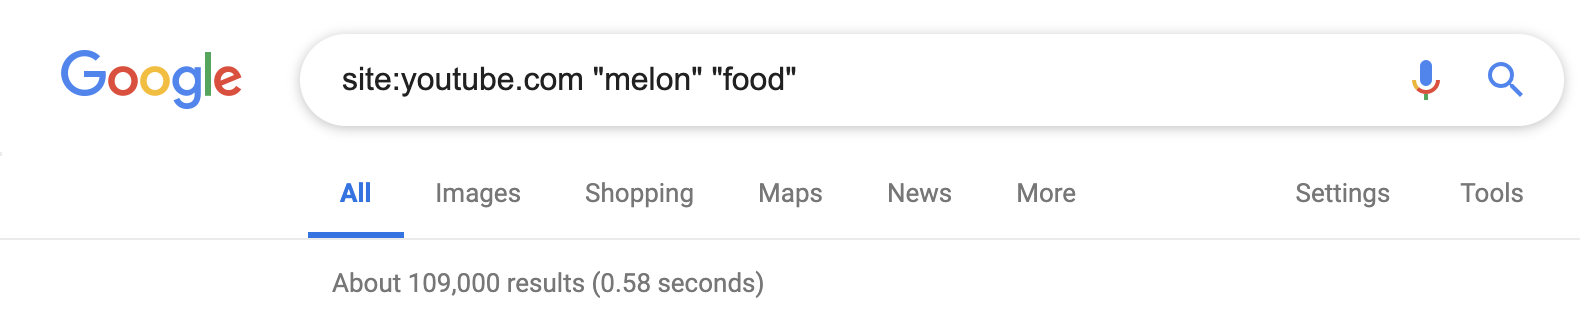
\includegraphics[width=350px]{youtube/melon.png}

        \vspace{1.5 cm}


        \paragraph{}
        \noindent Google Trends (Search) \\
        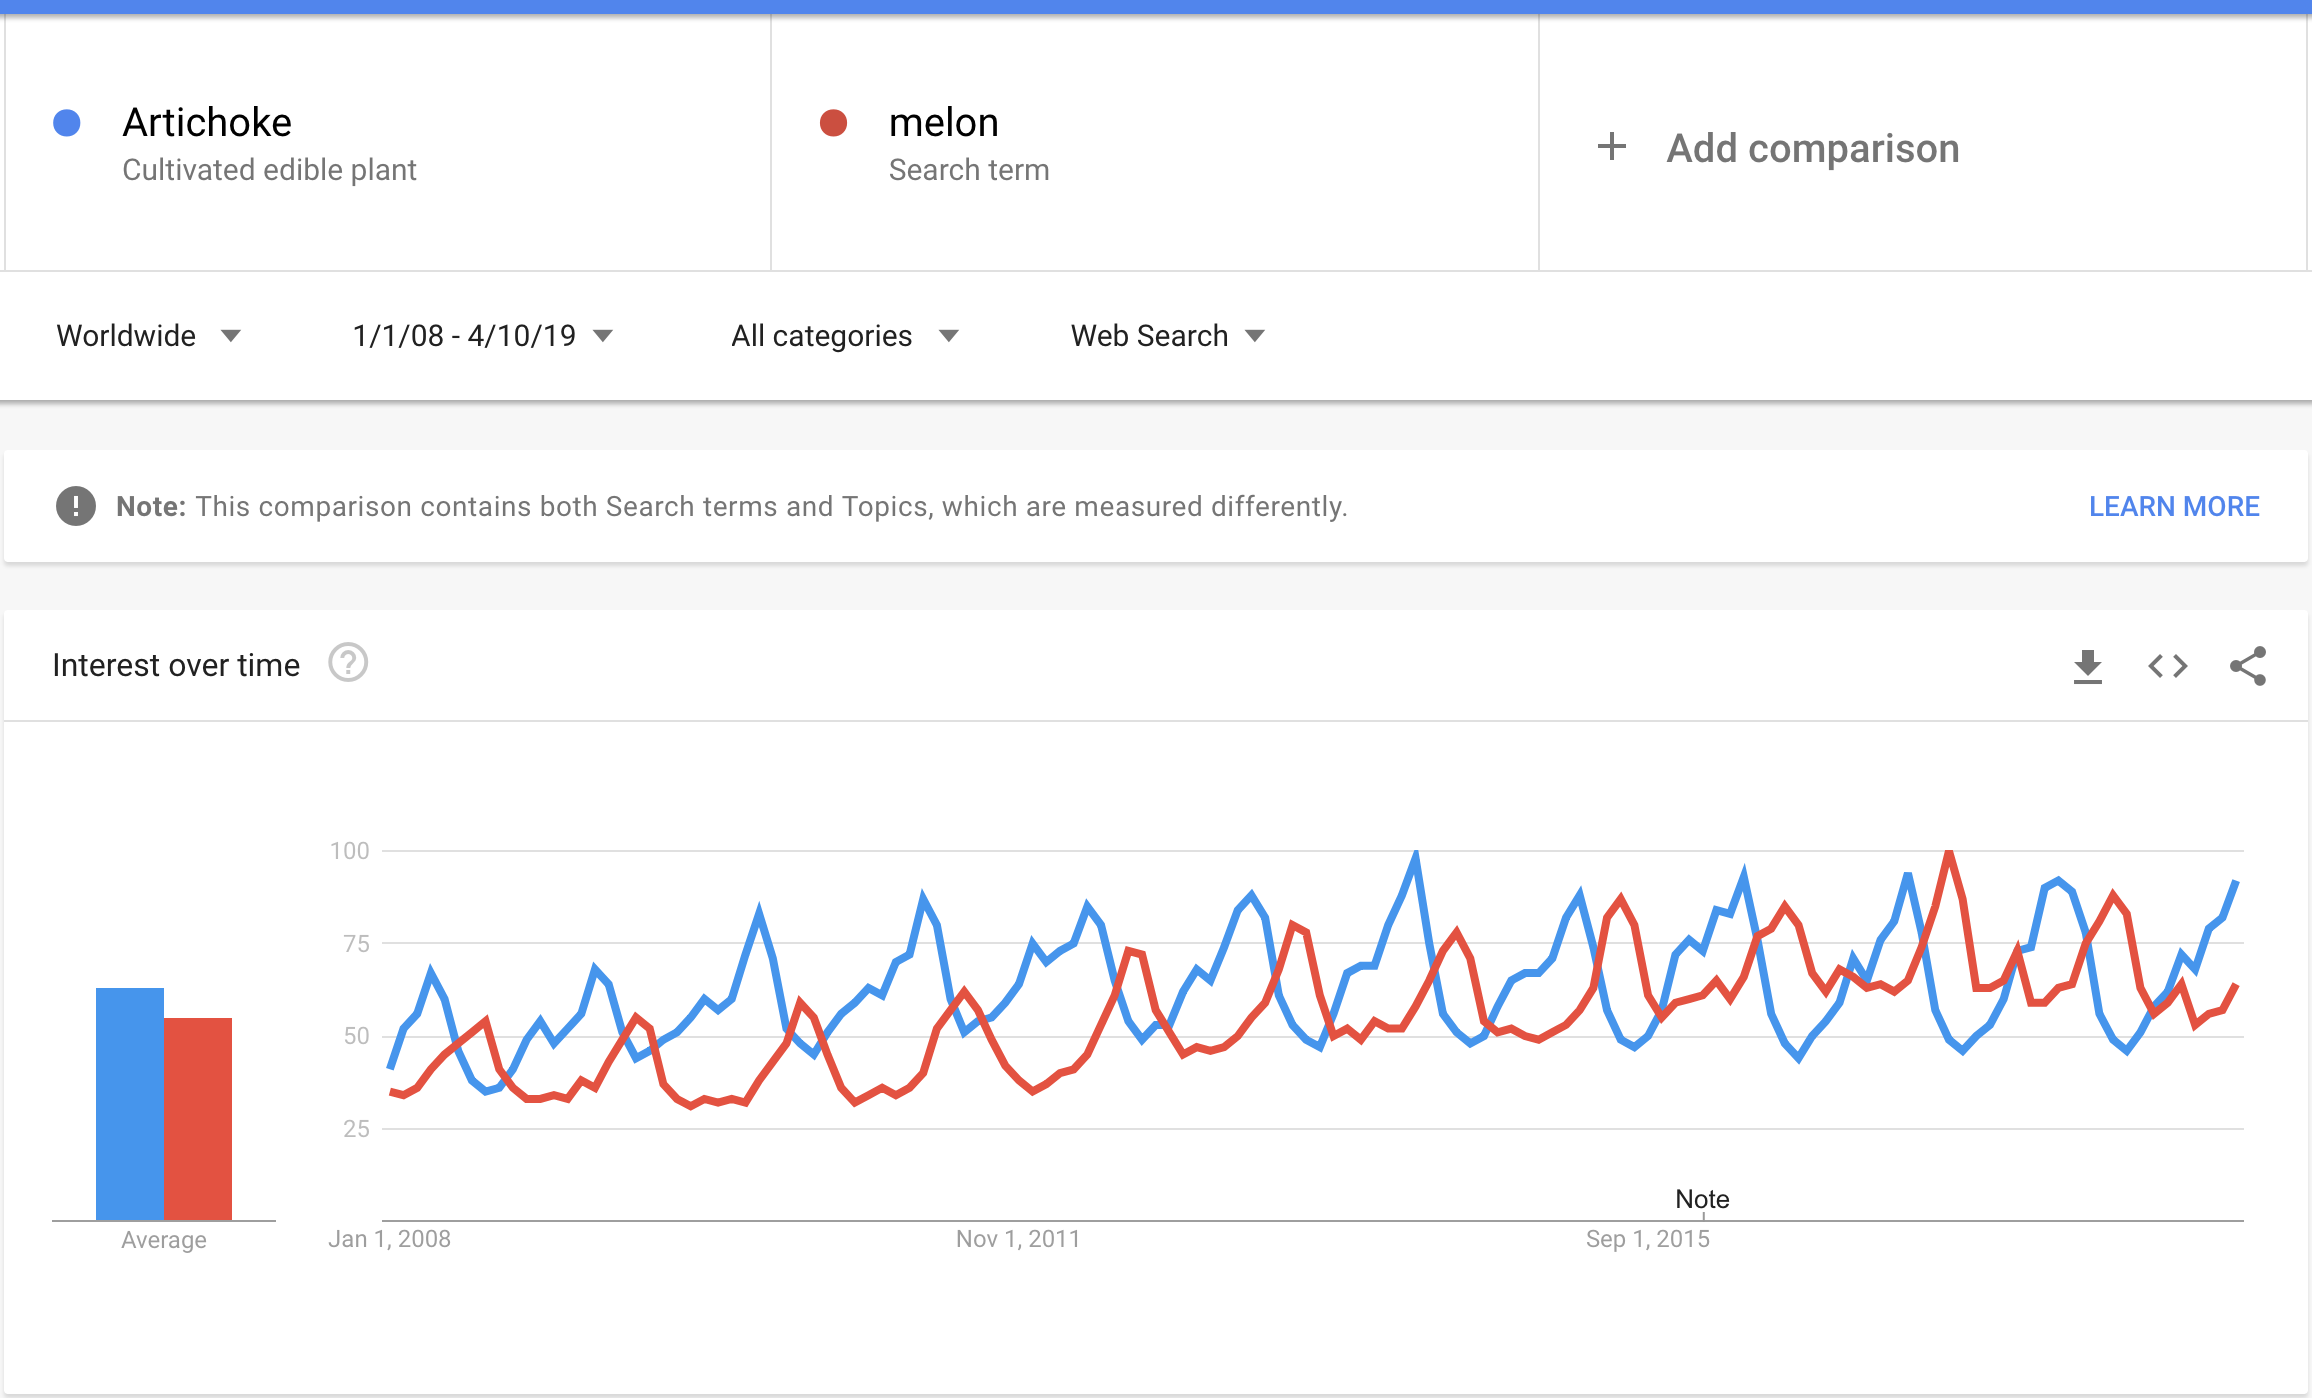
\includegraphics[width=350px]{google_trends/google.png}

        \vspace{1.5 cm}

        \paragraph{}
        \noindent Google Trends (Image) \\
        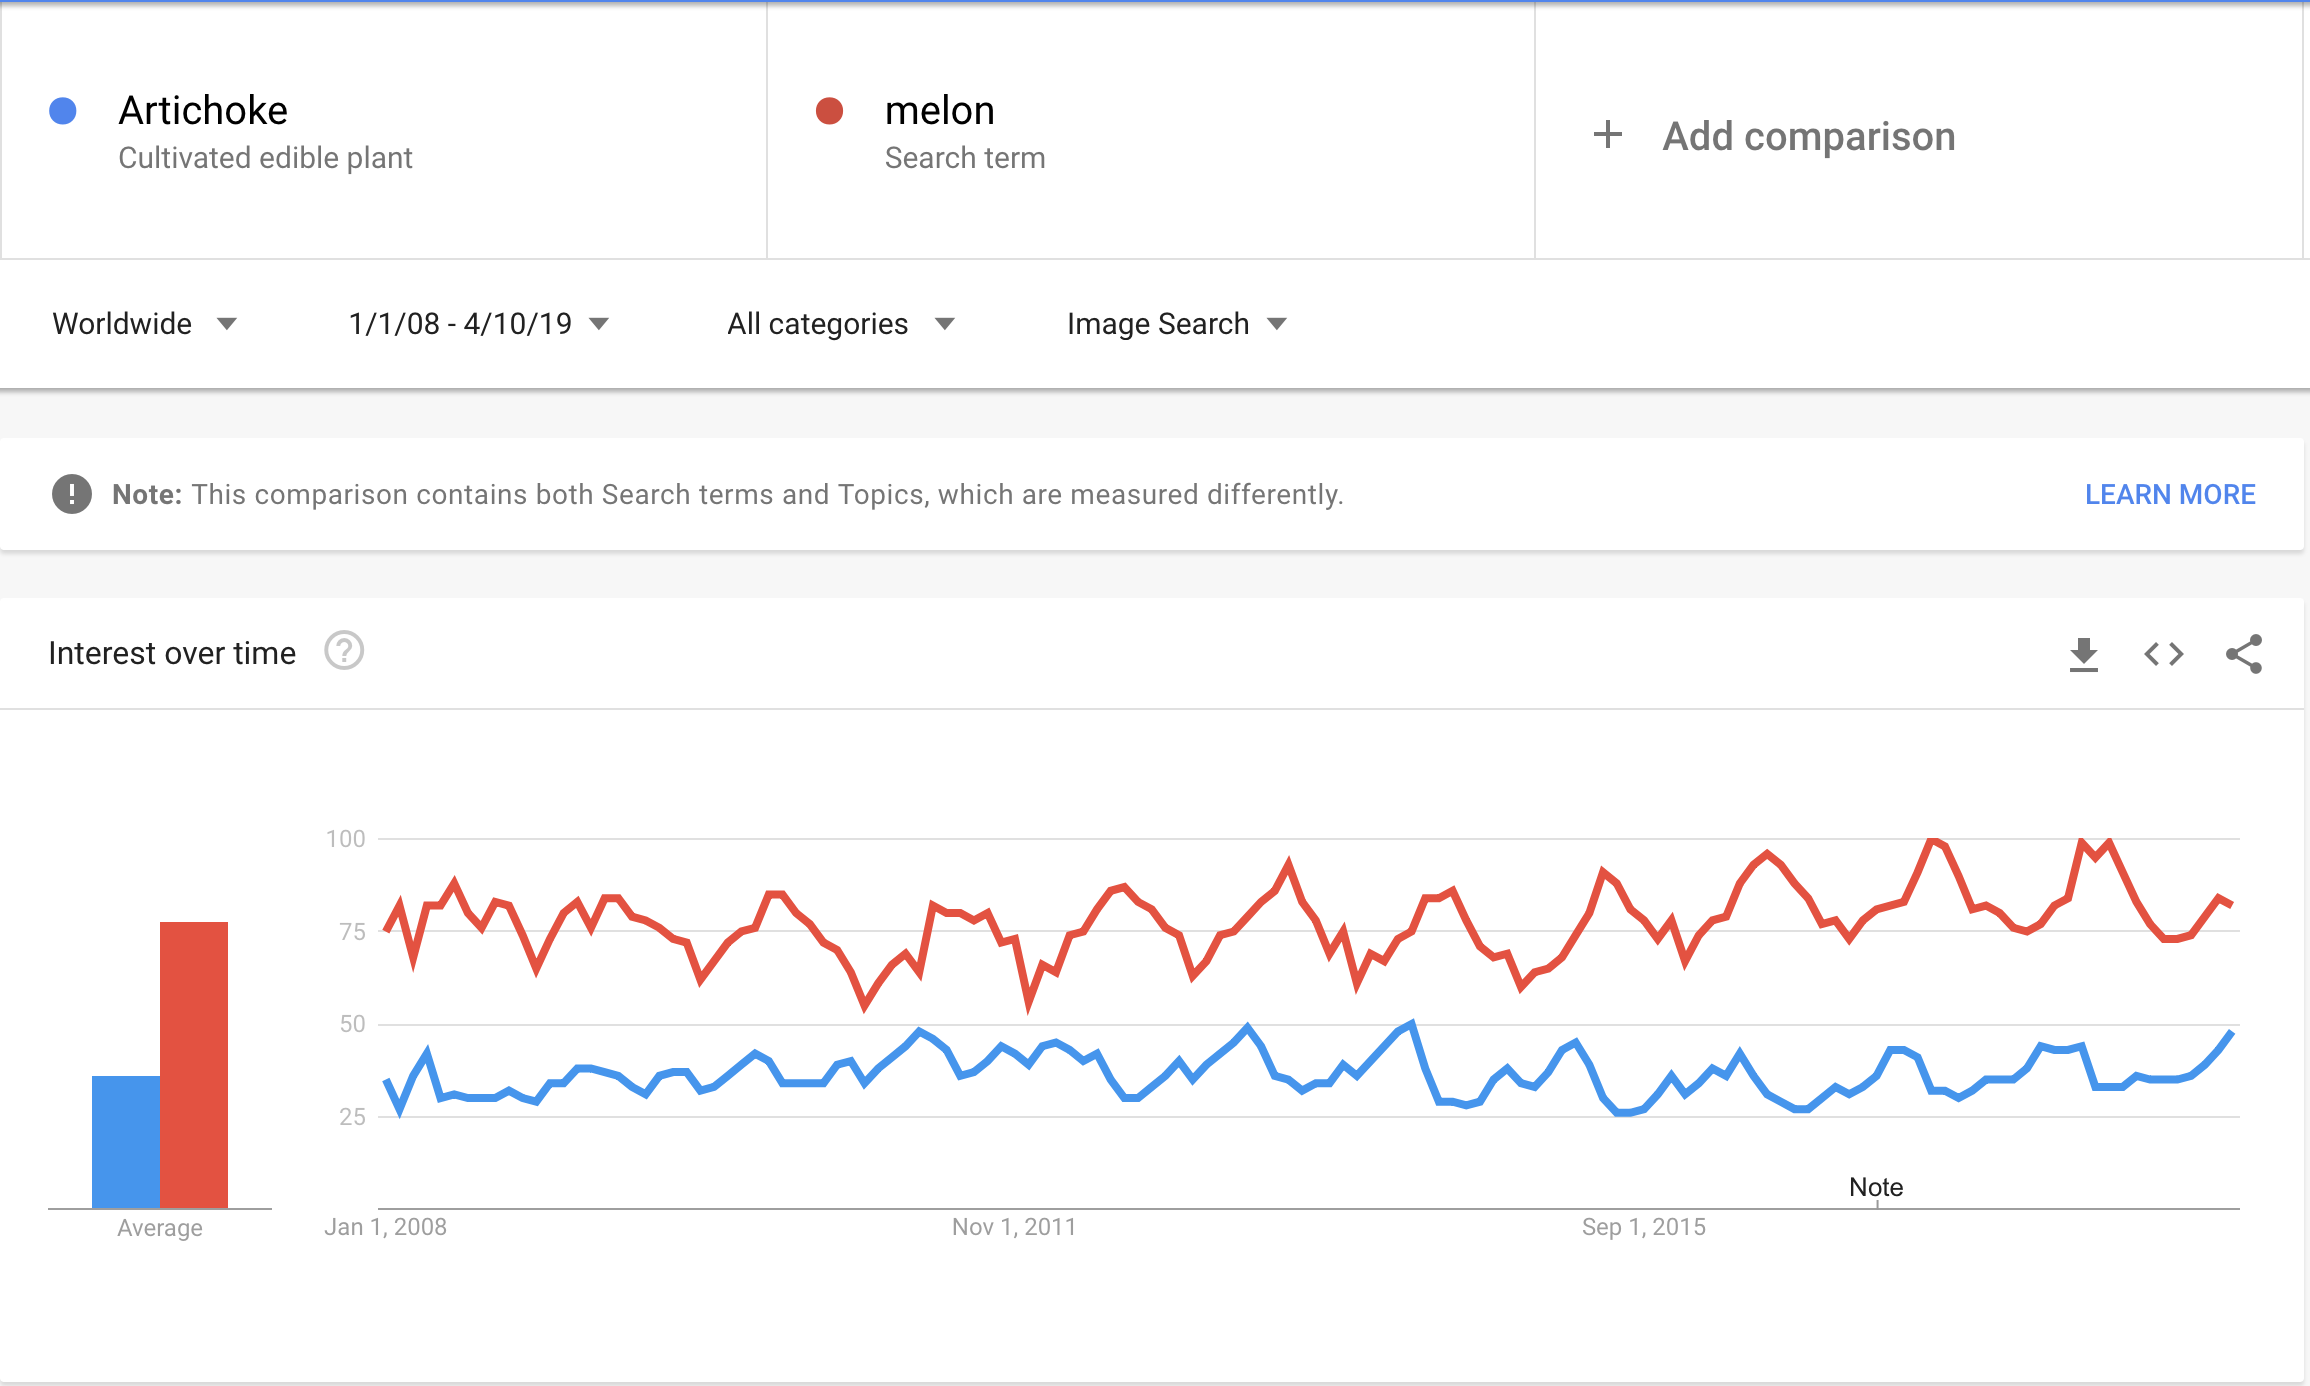
\includegraphics[width=350px]{trends/image.png}

      \subsubsection{Multiple Usages}
        \textbf{n/a}
      
      \subsubsection{Use in Sequences}
        \paragraph{}
        There are three notable linear sequences that the authors believe are of interest, namely the catch phrase ``okey dokey artichokey'', artichoke pizza, and artichoke dip.

        \begin{table}[h]
          \centering
          \begin{tabular}{P{5cm}P{5cm}}
          \hline
            Linear Sequence (Latin) & Emoji Representation          \\ \hline
            Okey dokey artichokey   & Okey dokey \artichoke{18px}   \\ \hline
            Okey dokey artichokey   & \thumbs{18px}\artichoke{18px} \\ \hline
            Artichoke dip           & \artichoke{18px}\bowl{18px}   \\ \hline
            Artichoke pizza         & \artichoke{18px}\pizza{18px}  \\ \hline
          \end{tabular}
          \caption{Images other than the artichoke are pulled directly from the Emoji 12.0 reference list on the Unicode website.}
          \label{linear-sequence}
        \end{table}
      
      \subsubsection{Breaking new ground}
        \paragraph{}
        The artichoke is a brand new vegetable not currently included or representable given the current Emoji 12.0 characters. It would also be the first thistle, ``the common name of a group of flowering plants characterized by leaves with sharp prickles on the margins'', added as an emoji. Given the unique appearance of the artichoke and its membership in the thistle group, the authors believe that this emoji would be ``breaking new ground''.

    \subsection{Image Distinctiveness}
        \paragraph{}
        The authors believe that the unique pointed shape of the artichoke's petals and it's overall fractal like structure make it easily recognizenizable at both small and large scales. This emoji stands out as unique in pictographic representation from the emoji in it's category, \texttt{food-vegtable}, as well as other emoji in the larger Emoji 12.0 standard.

    \subsection{Completeness}
      \textbf{n/a}
    \subsection{Frequently Requested}
      \textbf{n/a}

  \section{Selection Factors -- Exclusion}
    \subsection{Overly Specific}
        \paragraph{}
        The authors of this proposal believe that the artichoke is not overly specific. As the artichoke is one of the only edible thistles; It is also a popular ingredient in italian and american dishes for example artichokes alla Romana and artichoke dip respectively. The particular image could be drawn more generally to represent other thistles, as other members appear visually similar to the artichoke especially at small sizes. While flowering thistles could be achieved with a ZWJ between the artichoke and blossom emoji should a vendor see it as necessary.
    
    \subsection{Open-Ended}
        \paragraph{}
        As mentioned in the previous section the artichoke emoji could represent the larger thistle class, and artichoke was chosen for this proposal due to it's cultural significance as compared to other thistles.
    
    \subsection{Already Representable}
      \paragraph{}
      The authors of this proposal do not see a clear sequence of characters with or without a ZWJ that would adequately represent the artichoke. Due to its unique appearance the authors believe that the only logical way to represent it would be with a new character.

    \subsection{Logos, brands, UI icons, signage, specific people, specific buildings, deities.}
        \paragraph{}
        The artichoke has existed genetically longer than humans and thus its representation would be in no way linked to any human created mark or structure.

    \subsection{Transient}
        \paragraph{}
        The artichoke has been cultivated in italy for many hundreds of years and will likely continue to play a large and growing role in future cuisines. So the authors of this proposal do not find it likely given the Google Trend and historical data that the artichoke will fall out of favor in the near to long term future.
    
    \subsection{Faulty Comparison}
        \paragraph{}
        The authors do not believe that this proposal has outlined any arguments in favor of the artichoke emoji that were dependant on its comparison to other emojis outside the reference data.
    \subsection{Exact Images}
        \paragraph{}
        A Google Images search of ``artichoke clipart'' will demonstrate to the committee that there is no consensus on the visual representation of the artichoke, and the authors believe that it will be trivial to create house styles for the artichoke emoji that end users will still recognize as an artichoke.

    \subsection{Region Flags Without Code}
        \paragraph{}
        The authors do not believe that there are any specific visual representations of artichokes that are used as a flag, nor are they proposing it as one.

    
\end{document}